\documentclass{21kuur}

\title{UURIMISTÖÖ VORMISTAMINE \latex TARKVARAGA TALLINNA 21. KOOLI NÕUETE JÄRGI}
\author{Karl Kask}
\klass{XI klass}
\juhendaja{Siim Luha}

\begin{document}
\maketitle
\tableofcontents

\chapter*{SISSEJUHATUS}
\addcontentsline{toc}{chapter}{SISSEJUHATUS}
Peale mu algse teemavaliku kinnitamist võttis minuga ühendust kooli infotehnoloog ja väitis, et sellist uurimistööd pole koolil vaja ning soovitas mulle alternatiivi. Kuna väljapakutu minus erilist huvi ei tekitanud, otsustasin endale uue teema välja mõelda. Peale mitmeid vestlusi oma vennaga, kes on varem uurimistööid LaTeX tarkvaraga vormistanud, sain oma lõpliku uurimistöö teema sõnastatud.
\\\\LaTeX tarkvara võimaldab õpilasele sellise olukorra, kus ta peab sisestama vaid oma uurimistöö teksti ja kogu vormistus toimub automaatselt vastavalt nõuetele. Uurimistöö vormistamine võib olla keeruline ja aeganõudev osa töö koostamisest mitmeil põhjuseil. Esiteks on vormistamise nõuded erinevatel koolidel erinevalt määratletud. Seega ei saa informatsiooni vormistamise kohta teistest allikatest, kui kooli juhendist või juhendajalt. Teiseks võib kõikide nõuete täpne jälgimine ja reaalne kehtestamine olla aeglane ja liigselt tähelepanu nõudev protsess, sest seda peab tegema käsitsi. Pikaaegne vormistamise periood võib negatiivselt mõjuda töö sisule ja kvaliteedile.
\\\\Antud uurimistöö eesmärk on luua selline lahendus, kuhu õpilane peab sisestama ainult oma uurimistöö teksti ning vormistamine toimub automaatselt LaTeX tarkvara kaudu. Ühtlasi on eesmärgiks tutvustada LaTeX tarkvara ajalugu, sisu ja eeliseid uurimistöö vormistamisel. Innustada õpilasi kasutama LaTeX tarkvara oma uurimistöö vormistamisel, et nende töö kvaliteet ja sisu väärtus ei langeks vormistamise arvelt. 
\\\\Kolm uurimisküsimust on püstitatud uurimistöö eesmärgi täitmiseks. Mis on LaTeX tarkvara? Millised on LaTeX tarkvara positiivsed ja negatiivsed küljed võrreldes enamlevinud tekstiredaktoritega? Kuidas vormistada uurimistööd Tallinna 21. Kooli nõuete järgi LaTeX tarkvaraga?
\\\\Uurimistöö esimeses pooles tutvustatakse LaTeX tarkvara olemust, ajalugu ning positiivseid kui ka negatiivseid külgi. Teine pool on pühendatud LaTeX tarkvara kasutamisele, kus seletatakse täpselt lahti kogu uurimistöö LaTeX tarkvaraga vormistamise protsess.
\\\\Põhiliste allikatena kasutan LaTeX tarkvara juhend-raamatuid. Neist tähtsaim ja sisukaim „The LaTeX Companion”.

\chapter{TEOREETILINE TAUST}
TeX tarkvara on Donald Knuth'i loodud tavateksti kui ka muud visuaalset infot sisaldavate dokumentide loomise vahend. Knuth iseloomustas TeX tarkvara, kui imeilustae raamatute loomise vahendit - eriti, kui raamat sisaldab palju matemaatikat (Mittlebach \& Goossens, 2004: 1). 1990-ndate algul lõpetas Knuth tarkvara stabiilsuse huvides TeX-i arendamise. 1980-ndatel alustas Leslie Lamport LaTeX tarkvara arendust. LaTeX on dokumentide ettevalmistussüsteem, mis kasutab märgenduskeelt ja TeX programmi. LaTeX-i vahendid dokumendi loomise automatiseerimiseks teevad selle kasutamise lihtsamaks kui TeX-i kasutamise. LaTeX on tarkvarana kujunenud üheks peamiseks TeX-i kasutamise vahendiks. LaTeX-i filosoofia seisneb autorite vabadusel olla keskendunud sellele, millest nad kirjutavad ja mitte olla häiritud sellest, milline on kirjatöö visuaalne presentatsioon. LaTeX tarkvara kasutatakse memorandumite, nii äri kui ka isiklike kirjade, ajalehtede, artiklite ja raamatute vormistamiseks (Mittlebach \& Goossens, 2004: 1). LaTeX on põhiline keeruliste tabelite ja matemaatiliste valemite kujutamismeetod (Kopka \& Daly, 2012: 7). LaTeX tarkvara kasutatakse paljudes erinevates eluvaldkondades: nii teaduses, ajakirjanduses kui ka kunstis (Kopka \& Daly, 2012: 3). LaTeX on läbinisti vabavara. Selle arendus on lubatud avalikkuse kätte, tingimusel, et uue lahenduse nimi on muudetud (Kopka \& Daly, 2012: 3). 
\\\\LaTeX-i süsteem on struktureeritud pakettidesse, mille hulk sõltub dokumendi iseloomust ja keerukusest. Pakette on võimalik ka ise juurde luua ja sellega LaTeX-i laiendada. LaTeX dokumenti valmistades kirjeldab autor struktuuri märksõnadega nagu peatükk, osa, tabel, joonis, valem jms. LaTeX hoolitseb teksti ja muude elementide paigutuse ja peatükkide, valemite, tabelite ja piltide automaatse nummerdamise ning kasutatud kirjanduse viidete ning sisukorra eest.

\section{Miks LaTeX?}
LaTeX suurim erinevus teiste tekstiredaktoritega seisneb loogilises disainis. Enamlevinud tekstiredaktorid põhinevad visuaalsel disainil, mistõttu neid nimetatakse „WYSIWYG”(what you see is what you get) programmideks. Visuaalse disaini atraktiivsus seisneb kasutaja võimaluses muuta oma dokumendi välimust töölaual otseselt. Neid programme on iseloomustatud ka lausega „what you see is all you've got”, millest tuleb välja ka nende programmide suurim nõrkus (Lamport, 1994: 7). Loogilise disaini võimsus seisneb disaini piiramatuses ja mitmete samasuguste elementide automaatses üheaegses muutmises. Üks suurimaid LaTeX tarkvara eeliseid on vormistuse eraldamine sisust klassi faili abil. See tähendab, et sama vormistuse peale võib kirjutada lõputuid erinevaid töid, ning sisu vastaks ikka nõuetele. Visuaalse disaini korral peab kõik tööd eraldi vormistama, sest seal peab kõik nõuded uuesti paika panema ja sisestama. LaTeX tarkvara negatiivne külg on vajadus klassi faili või siis piisavate teadmiste järele, et vormistamisega TeX programmis hakkama saada. Üldjuhul on ülikoolidel klassi fail olemas, ning seda ei pea ise looma. LaTeX tarkvaraga on võimalik ühtlustada dokumentide vormistamist institutsioonisde siseselt.

\chapter{METOODIKA}
Oma uurimistöö käigus uurin TeX ja LaTeX tarkvara ajalugu, kasutamisalasid ning positiivseid ja negatiivseid külgi. Oma uurimistöö praktilises osas arendan välja toimiva lahenduse uurimistöö vormistamiseks LaTeX tarkvaras ja kirjeldan üksikasjalikult protsessi. Tutvun põhjalikult kooli uurimistöö juhendiga ning LaTeX dokumentatsiooniga\footnote{http://en.wikibooks.org/wiki/LaTeX}. Proovin luua võimalikult võimeka klassi faili, et tex faili peaks võimalikult vähe sisestama koodi, mis on seotud töö vormistamisega. Klassi faili lisan tööle lisana.

\chapter{UURIMISTÖÖ VORMISTAMINE \latex TARKVARAGA}
Uurimistöö vormistamiseks LaTeX tarkvaraga on vaja arvutile installeerida mõni TeX programm. Näiteks MikTeX. Samuti on vaja kooli nõuetele vastavat klassi faili. Tallinna 21. Kooli uurimistööd võib vormistada selle uurimistöö käigus loodud 21kuur.cls faili kasutades. Uurimistöö tex faili kirjutamist saab alustada, kui fail on salvestatud samasse kausta, kus asub klassi fail. Samasse kausta tuleb ka salvestab programm ka pdf faili. Tex faili sisu sisestatakse Texworks programmi aknasse ning ülevalt vasakult rippmenüüst valitakse pdfLaTeX + MakeIndex + BibTeX. Sisestatud koodi välundit on võimalik iga hetk kontrollida üleval vasakul oleva rohelise nupu vajutamisel. Nupu vajutamisel loob programm pdf faili, milleks on ka lõplik uurimistöö fail.
\section{Üldine tex faili struktuur}
TeX koodis on põhiliseks elemendiks tagurpidi kaldkriips. Sellega alustatakse käske, alustatakse uut rida ja päästetakse veaohtlikke elemente. Kõik käsud kirjutatakse väikeste tähtedega. Kommentaaride tegemiseks kasutatakse protsendi märki. Programm ei loe rea lõpuni teksti, mis on peale protsendi märki. Kommentaare võib kasutada tex faili sisu selgitamiseks. Kommentaarides ei pea veaohtlikke elemente päästma.

LaTeX failide kood algab tavapäraselt dokumendi klassi nimetamisega. Antud juhul on klassiks 21kuur.
\begin{verbatim}
\documentclass{21kuur} % See on kommentaar. Seda teksti 
programm ei loe.
\end{verbatim}
LaTeX failis tähistavad dokumendi sisu algust ja lõppu vastavalt begin ja end käsud. Argumendiks on document.
\begin{verbatim}
\begin{document}
\end{document}
\end{verbatim}
LeTeX failis saab uuele leheküljele minna newpage käsuga. Käsk sisestatakse peale sisu, mida tahetakse jätta eelmisele leheküljele.
\begin{verbatim}
\newpage
\end{verbatim}
Peatükkide ja alapeatükkide pealkirju luuakse vastavalt chapter ja section käskudega. Alapeatükkide alapealkirjad tähistatakse subsection käsuga. Peale käsku kirjutatakse looksulgude sisse pealkiri suurte tähtedega vastavalt juhendile. Alapaelkirjadel peab suur olema vaid esimene täht. Ilma numbrita pealkirja saab peale käsku tärni lisamisega. Ilma numbrita peatükid sisestatakse sisukorda käsitsi. Selleks kasutatakse kohe järgmisel real addcontentsline käsku, mille esimeseks argumendiks on toc, teiseks argumendiks chapter ja kolmandaks argumendiks peatüki nimi.
\begin{verbatim}
\chapter{PEALKIRI}
\section{Alapealkiri}
\subsection{Ala-alapealkiri}
\chapter*{NUMMERDAMATA PEALKIRI}
\addcontentsline{toc}{chapter}{NUMMERDAMATA PEALKIRI}
\end{verbatim}
Lehekülje number eemaldatakse thispagestyle käsuga. Argumendiks on empty. Käsk asetatakse peale chapter käsku. Ilma leheküle numbrita on näiteks lisade ja kasutatud materjalide leht. Käsku ei pea kasutama tiitellehel ega sisukorra lehel, sest automaatne nummerdamine algab alates esimeset chapter käsust.
\begin{verbatim}
\chapter{ILMA LEHEKÜLJE NUMBRITA LEHEKÜLJEL ASETSEVA PEATÜKI 
PEALKIRI}
\thispagestyle{empty}
\end{verbatim}

\section{Tiitllehe ja sisukorra loomine}
Tiitellehe loomiseks määratakse enne dokumendi sisu algust tiitellehel olev sisu. Seda tehakse käskudega title, argumendiks uurimistöö pealkiri suurte tähtedega vastavalt juhendile, author, argumendiks uurimistöö koostaja nimi, klass, argumendiks koostaja klass, juhendaja, argumendiks juhendaja nimi. Asutuse nimi, asukoht, töö liik ja aasta lisatakse automaatselt.
\begin{verbatim}
\title{UURIMISTÖÖ NIMI}
\author{Koostaja Nimi}
\klass{koostaja klass nt. "XI klass"}
\juhendaja{Juhendaja Nimi}
\end{verbatim}
Tiitelleht lisatakse dokumendi sisse maketitle käsuga, millel argument puudub. Tavaliselt on tiitleleht kohe peale dokumendi alustamise käsku.
\begin{verbatim}
\maketitle
\end{verbatim}
Sisukorra loomiseks sisestatakse tableofcontents käsk ilma argumendita ning sisukord luuakse programmi poolt automaatselt. Tavaliselt asetseb käsk sisukorra loomiseks kohe peale tiitlelehe loomise käsku.
\begin{verbatim}
\tableofcontents
\end{verbatim}

\section{Töö sisu sisestamine}
Töö sisu sisestatakse kohe peale pealkirja käsku järgmisele reale lihtsa tekstina. Rööpjoondus ja sõnade poolitamisega toimub automaatselt. Reavahetust tekitatakse kaksik tagurpidi kaldkriipsuga. Uue paragrahvi loomiseks sisestatakse teksti vahele neli tagurpidi kaldkriipsu.
\begin{verbatim}
\chapter{PEALKIRI}
Siin on esimene paragrahv.\\\\Siit algab järgmine paragrahv.\\
Siit algab järgmisel real olev tekst.
\end{verbatim}
Teksti sisust päästetakse tagurpidi kaldkriipsuga veaohtlikud elemendid, mida programm võib lugeda käsuna. Mõne elemendi saamiseks on vaja sisestada käsk. Veaohtlikud elemendid on: \&, \%, \$, \#, \_, \{, \}, \textasciitilde, \textasciicircum, \textbackslash. Koodinäitena on toodud eelmine lause sellisena, nagu ta tex failis kirjutatakse ning näide, kuidas päästa elementi teksti siseselt.
\begin{verbatim}
Veaohtlikud elemendid on: \&, \%, \$, \#, \_, \{, \}, 
\textasciitilde, \textasciicircum, \textbackslash.

(Kopka \& Daly, 2012: 3)
\end{verbatim}

\section{Kasutatud materjalid}
Kasutatud materjalide leht täidetakse vastavalt kooli juhendile käsitisi. Pealkiri luuakse chapter käsuga, millele on listaud tärn, et nummerdamist ära kaotada. Erinevad teosed peavad algama uuelt realt. Reavahetuseks kasutatakse neljakordset tagurpidi kaldkriipsu. Näitena on kasutatud osa selle uurimistöö kasutatud materjalidest. Kasutatud materjalide lehel kaotatakse lehekülje number thispagestyle käsuga, mille argumendiks on empty.
\begin{verbatim}
Kopka, H., Daly, P. W. (2012). Guide to LaTeX. 4. tr. Boston: 
Addison-Wesley % esimene teos
\\\\Lamport, L. (1994). LaTeX: A Document Preparation System. 
2. tr. USA: Addison-Wesley

\thispagestyle{empty}
\end{verbatim}

\section{Tabelid, joonised, valemid ja loetelud}
Tabeli sisestamist alustatakse begin käsuga mille esimeseks argumendiks on tabular ja teiseks argumendiks tabeli kujundust määravad elemendid. Trafaretsemad teise argumendi elemendid on tähed r, l, c ning püstkriips. Argumendis esimene element määrab kõige vasakpoolsema veeru joonduse. Viimane element määrab kõige parempoolsema veeru joonduse. Keskmised elemendid määravad joonduse vastavalt sellel veerul, mitmendad elemendid nad argumendis on. Täht r tähistab parempoolset joondust, täht l vasakpoolset joondust ja täht c keskjoondust. Püstkriipse kasutatakse vertikaaljoonte loomiseks veergude vahele. Püstkriipsud asetatakse veergude joondust tähistavate elementide vahele. Kõik elemendid teises argumendis on eraldatud tühikuga. Tabelit lõpetatakse end käsuga, mille argumendiks on tabular. Tabeli sisu kirjutatakse begin ja end käskude vahele. Horisontaaljooni luuakse käsuga hline, millel pole argumente. Kahte veergu eristatakse \& sümboliga. Rida vahetatakse topelt tagurpidi kaldkriipsuga. Kõik elemendid on eraldatud tühikuga. Veergude ja ridade suurused määratakse automaatselt. Tabelitele lisatakse pealkirju captionof käsuga, mille esimeseks argumendiks on table ja teiseks argumendiks pealkiri. Numeratsioon toimub automaatselt. Keerukamate tabelite loomist selgitatakse põhjalikumalt LaTeX dokumentatsioonis\footnote{http://en.wikibooks.org/wiki/LaTeX/Tables}. Näitena on toodud tabel ja sellele vastav LaTeX kood.
\captionof{table}{Näite tabel.}
\begin{tabular}{| l | c | r |}
  \hline
  (1. rida 1. veerg) & (1.rida 2. veerg) & (1. rida 3. veerg) \\ \hline
  (2. rida 1. veerg) & (2. rida 2. veerg) & (2. rida 3. veerg) \\ \hline
	(3. rida 1. veerg) & (3. rida 2. veerg) & (3. rida 3. veerg) \\
	\hline
\end{tabular}\\
\begin{verbatim}
\captionof{table}{Näite tabel.}
\begin{tabular}{| l | c | r |}
	\hline
	(1. rida 1. veerg) & (1.rida 2. veerg) & (1. rida 3. veerg)
	 \\ \hline
	(2. rida 1. veerg) & (2. rida 2. veerg) & (2. rida 3. veer
	g) \\ \hline
	(3. rida 1. veerg) & (3. rida 2. veerg) & (3. rida 3. veerg) \\
	\hline
\end{tabular}
\end{verbatim}
Jooniste lisamiseks kasutatakse käsku includegraphics, mille järel tuleb nurksulgudes määrata joonise suurus ning mille argumendiks on pildi nimetus ilma faililaiendita. Pealkiri lisatakse käsuga captionof, mille esimeseks argumendiks on figure ja teiseks argumendiks pealkiri. Näites toodud joonise laius on 2,5 sentimeetrit.
\captionof{figure}{Tibu.}
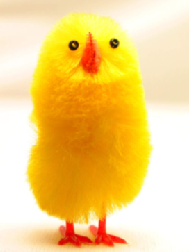
\includegraphics[width=2.5cm]{Chick1}
\begin{verbatim}
\captionof{figure}{Tibu.}
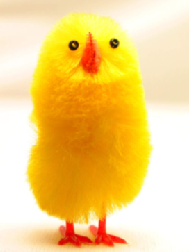
\includegraphics[width=2.5cm]{Chick1}
\end{verbatim}
Valemite tekstisisesel kujutamisel kasutatakse \$ sümbolit ning tekstivälisel kujutamisel topelt \$ sümbolit. Sümbolit kasutatakse valemi alguse kui ka lõpu tähistamiseks. Erinevate tehtemärkide kohta saab informatsiooni dokumentatsioonist\footnote{http://en.wikibooks.org/wiki/LaTeX/Mathematics}.
$$k_{n+1} = n^2 + k_n^2 - k_{n-1}$$
\begin{verbatim}
$$k_{n+1} = n^2 + k_n^2 - k_{n-1}$$
\end{verbatim}
Loetelusid alustatakse begin käsuga, mille argumendiks võib olla enumerate või itemize. Argumenti enumerate kasutates loob programm nummerdatud loetelu ning argumenti itemize kasutades loob programm nummerdamata loetelu. Loetelu trepitakse analoogselt sellele, millist tulemust soovitakse loetelus näha.
\begin{enumerate}
  \item Ese 1
  \begin{enumerate}
    \item Alaese 1
    \begin{itemize}
    	\item Nummerdamata ese 1
    	\item Nummerdamata ese 2
    \end{itemize}
    \item Alaese 2
  \end{enumerate}
  \item Ese 2
  \item Ese 3
\end{enumerate}
\begin{verbatim}
\begin{enumerate}
  \item Ese 1
  \begin{enumerate}
    \item Alaese 1
    \begin{itemize}
    	\item Nummerdamata ese 1
    	\item Nummerdamata ese 2
    \end{itemize}
    \item Alaese 2
  \end{enumerate}
  \item Ese 2
  \item Ese 3
\end{enumerate}
\end{verbatim}

\section{Viitamine}
Viited kasutatud materjalidele kirjutatakse teksti sisse käsitsi vastavalt juhendile. Joonealused viited sisestatakse käsuga footnote, mille argumendiks on viite sisu.
\begin{verbatim}
Tekst, millel on lisatud joonealune viide.\footnote{Viite sisu}
\end{verbatim}

\section{Lisad}
Lisade pealkirjana kasutatakse chapter käsku mille lõppu on pandud nummerdamise kaotamiseks tärn. Lisadel kaotatakse lehekülje number thispagestyle käsuga, mille argumendiks on empty.
\begin{verbatim}
\thispagestyle{empty}
\end{verbatim}

\chapter{TULEMUSED JA ANALÜÜS}
Lõpliku klassi failiga täitsin üldmääral oma uurimistöö peamise eesmärgi, milleks oli sellise lahenduse loomine, et õpilane peaks sisestama vaid oma uurimistöö sisu ning kogu vormistus toimuks automaatselt. Peale mõne koodirea on selline lahendus saavutatud. Uurimistöö vormistaja peab sisukorda käsitsi lisama vaid nummerdamata peatükid. Selles uurimistöös toodud juhendit järgides on võimalik uurimistöö üldjuhul automaatne vormistus. Samuti on olemas LaTeX tarkvara tutvustav teoreetiline osa, kus on põhjendatud selle eelised ning negatiivsed küljed võrreldes enamlevinud tekstiredaktoritega ning ülevaade LaTeX ning TeX tarkvara ajaloost. Seega on uurimistöö eesmärgid täidetud ning uurimisküsimustele vastatud. 
\chapter*{KOKKUVÕTE}
\addcontentsline{toc}{chapter}{KOKKUVÕTE}
Esimesele kahele uurimisküsimusele on vastatud esimeses peatükis ning kolmandale on vastatud kolmandas peatükis. Töö praktilises osas suutsin välja aretada piisavalt võimeka klassi faili, et täita uurimistöö eesmärk. Klassi faili loomine võttis oodetust kauem aega ning oli keerulisem, kui oletasin. Kuid üldjuhul on tulemus piisav. Klassi faili on tulevikus võimalik täiustada ning uuendada. Samuti toon välja ettepaneku täiustada kooli vormistamise juhendit, et sealt ei puuduks informatsioon tabelite, jooniste jm korrektse vormistamise kohta.

\chapter*{KASUTATUD MATERJALID}
\addcontentsline{toc}{chapter}{KASUTATUD MATERJALID}
Kopka, H., Daly, P. W. (2012). Guide to LaTeX. 4. tr. Boston: Addison-Wesley
\\\\Lamport, L. (1994). LaTeX: A Document Preparation System. 2. tr. USA: Addison-Wesley
\\\\Mittelbach, F., Goossens, M. (2004). The LaTeX Companion. 2. tr. Massachusetts: Addison-Wesley
\\\\LaTeX. (2013). LaTeX tarkvara dokumentatsioon. [en] http://en.wikibooks.org/wiki/LaTeX \\(31.10.2013).
\thispagestyle{empty}
\chapter*{LISA 1 KLASSI FAIL}
\thispagestyle{empty}
\addcontentsline{toc}{chapter}{LISA 1 KLASSI FAIL}
\begin{verbatim}
\NeedsTeXFormat{LaTeX2e}
\ProvidesClass{21kuur}[2013/10/24 21.kooli uurimustöö 
vormistuse klass]

\LoadClass[12pt]{report}  % kasuta standardset report klassi 
alusena.

% Lehe asetus.
\usepackage{geometry}
\geometry{top=2.50cm, bottom=2.50cm, left=3cm, right=2cm}
\geometry{paperwidth=210mm, paperheight=297mm} 
\geometry{textwidth=160mm, textheight=247mm, headheight=0cm, 
headsep=0cm}

\usepackage[utf8]{inputenc}
\usepackage[T1]{fontenc}

\usepackage[estonian]{babel} % Eesti keel vaikimisi keeleks.

\usepackage{tocbibind}

% Peatükid algavad uuelt lehelt.
\usepackage{etoolbox}
%\patchcmd{\chapter}{\if@openright\cleardoublepage\else\
clearpage\fi}{}{}{}

% Leheküljenumbrid algavad pärast esimest pealkirja, kuid 
pealkirjaga leht on tühi.
\renewcommand\thepage{}
\newtoggle{nummerdamelehti}
\togglefalse{nummerdamelehti}

% Käsk nummerdamise alustamiseks.
\newcommand{\nummerdame}{%
  \iftoggle{nummerdamelehti}{}{%
    \renewcommand\thepage{\arabic{page}}%
    \toggletrue{nummerdamelehti}%
    \thispagestyle{empty}%
  }
}

% Esimese peatüki juures nummerdamise alustamine.
\end{verbatim}
\pagenumbering{gobble}
\begin{verbatim}
\patchcmd{\addchap}{\secdef}{\nummerdame\secdef}{}{}
\pretocmd{\chapter}{\nummerdame{}}{}{}

% tocloft pakett.
\usepackage{tocloft}

% Sisukorra pealkirja asetus.
\setlength{\cftbeforetoctitleskip}{-16pt}
\setlength{\cftaftertoctitleskip}{20pt}

% Jaotuste numbrite taga punktid.
\renewcommand{\cftchapaftersnum}{.}
\renewcommand{\cftsecaftersnum}{.}
\renewcommand{\cftsubsecaftersnum}{.}
\renewcommand{\cftsubsubsecaftersnum}{.}

% Kujutame kõikide jaotuste pealkirju.
\setcounter{tocdepth}{99}
% Nummerdus
\setcounter{secnumdepth}{99}

% Sisukorra pealkirja font.
\renewcommand{\cfttoctitlefont}{\fontsize{16pt}{19.2pt}
\selectfont}

% Sisukorra  pealkirjas suured tähed.
\addto{\captionsestonian}{\renewcommand*{\contentsname}
{SISUKORD}}

% 1.5 reavahetus.
\usepackage{setspace}
\onehalfspacing

% Times New Roman kõikjal.
\usepackage{times}

% Eemaldab paragrahvidel taande ja teeb nende vahele tühja rea.
\usepackage[parfill]{parskip}

% titlesec pakett.
\usepackage{titlesec}

% Tiitellehe kujundus
%% Tiitellehe genereerimine
% Eestikeelsed muutujad.
\def\klass#1{\gdef\@klass{#1}}
\def\juhendaja#1{\gdef\@juhendaja{#1}}
\def\asutus#1{\gdef\@asutus{#1}}
\def\paber#1{\gdef\@paber{#1}}
\def\koht#1{\gdef\@koht{#1}}

% Vaikeväärtused
\paber{Uurimist\"o\"o}
\asutus{Tallinna 21. Kool}
\koht{Tallinn}

% Kood tiitellehe genereerimiseks.
\renewcommand{\maketitle}{\newpage
        \thispagestyle{empty}
        \vspace*{-1cm}
        \begin{center}
        {\fontsize{14pt}{16.8pt}\selectfont\expandafter
        {\@asutus}} \\
        \end{center}
        \vskip1in

        \vfill

        \begin{center}
                {\fontsize{20pt}{24pt}\selectfont\bfseries
                \expandafter{\@title}}
        \end{center}
        {\fontsize{14pt}{16.8pt}\selectfont\centerline{\@paber}}

        \vskip.5in
        \vfill
        
        \begin{flushright}
                {\fontsize{14pt}{16.8pt}\selectfont\expandafter
                {\@author} \expandafter{\@klass}} \\
                Juhendaja: \expandafter{\@juhendaja}
        \end{flushright}
        \vskip.5in

        \vfill
        {\fontsize{14pt}{16.8pt}\selectfont\centerline{\@koht{} 
        \the\year}}%
        \clearpage
        }

% Peatüki pealkirja kujundus.
\titleformat{\chapter}[hang]
  {\fontsize{16pt}{19.2pt}\selectfont}
  {\thechapter. } % Etiketi formaat
  {0pt} % Märgise ja pealkirja vahe.
  {\uppercase} 
  [] 

\titlespacing{\chapter}
  {0pt} % Vasakult
  {*0} % Vertikaal enne
  {*2} % Vertikaal peale

% Peatüki eelne vahe.
\def\ttl@mkchap@i#1#2#3#4#5#6#7{%
    \ttl@assign\@tempskipa#3\relax\beforetitleunit
    \vspace{\@tempskipa}% Eelmalda pealne \vspace.
    \global\@afterindenttrue
    \ifcase#5 \global\@afterindentfalse\fi
    \ttl@assign\@tempskipb#4\relax\aftertitleunit
    \ttl@topmode{\@tempskipb}{
        \ttl@select{#6}{#1}{#2}{#7}}
    \ttl@finmarks
    \@ifundefined{ttlp@#6}{}{\ttlp@write{#6}}}

% Alapeatüki pealkirja kujundus.
\titleformat{\section}[hang]
  {\fontsize{14pt}{16.8pt}\selectfont\bfseries}
  {\thesection. }
  {0pt}
  {}
  [] 

% Alapeatüki pealkirja kujundus.
\titlespacing{\section}
    {0pt} % Vasakult
    {*1} % Vertikaal enne
    {*1} % Vertikaal peale

% Alapeatüki alapealkirja kujundus.
\titleformat{\subsection}[hang]
  {\fontsize{12pt}{14.4pt}\selectfont\bfseries}
  {\thesubsection. }
  {0pt}
  {}
  [] 

%% Tabelid ja joonised.

% Tabelite ja jooniste numbrid ilma koolonita.
\usepackage{caption}
% Kõik pealkirjad vasakjoondusega.
\captionsetup{justification=justified,singlelinecheck=false}

% Joonis vahetult seda kirjeldava teksti juures ehk sama 
alapeatüki sees.
\usepackage[section]{placeins}

% Pealkirjad pealkirjade stiili.
\newcommand{\trkcaptionsetup}{\captionsetup{labelformat=simple, 
labelsep=period, labelfont=bf, font=bf}}
\trkcaptionsetup
% Pealkirjad allika moodi.
\newcommand{\captionstosource}{\captionsetup{labelformat=simple, 
labelsep=period, font=normalfont}}
% Allika lisamine joonisele.
\newcommand{\allikas}[1]{\vspace{-3mm}\captionstosource\caption*
{Allikas: #1}\trkcaptionsetup}

% Tabelite, jooniste ja valemite läbiv numeratsioon.
\usepackage{chngcntr}
\counterwithout{figure}{chapter}
\counterwithout{table}{chapter}
\counterwithout{equation}{chapter}
\counterwithout{footnote}{chapter}

% graphicx pakett jooniste sisestamiseks.
\usepackage{graphicx}

% xspace pakett, ning käsk nime LaTeX stiliseeritud kujutamiseks
\usepackage{xspace}
\newcommand{\latex}{\LaTeX\xspace}

% Joonealuste viidete tähestikuline nummerdamine.
\renewcommand{\thefootnote}{[\alph{footnote}]}

% Joonealuste viidete nummerdamise lähtestamine.
\usepackage{perpage}
\MakePerPage{footnote}

\end{verbatim}

\end{document}
